\section{Clustervalidierungsverfahren}

\begin{defi}{Clustervalidierungsverfahren}
    \emph{Clustervalidierungsverfahren} bewerten die Qualität von Clusterings (Partitionen) und ermöglichen so das Einstellen von Hyperparametern\footnote{Beispiel: Anzahl $K$ der Cluster bei K-Means}.

    Man unterscheidet zwischen drei Arten:
    \begin{enumerate}
        \item \emph{Tests auf Abwesenheit von Clusterstruktur}
              \begin{itemize}
                  \item häufig in Forschungskontexten, selten in der Praxis
                  \item Tests gegen typische Nullhypothesen
                        \begin{itemize}
                            \item Daten liegen zufällig verteilt im Merkmalsraum (\emph{Uniformitätshypothese})
                            \item Daten wurden aus unimodaler Verteilung gezogen (\emph{Unimodale Nullhypothese})
                        \end{itemize}
              \end{itemize}
        \item \emph{Externe Clustervalidierung}
              \begin{itemize}
                  \item Kriterien, die auf externen Informationen über die wahre Clusterzugehörigkeiten basieren
              \end{itemize}
        \item \emph{Interne Clustervalidierung}
              \begin{itemize}
                  \item Kriterien, die allein auf den Daten basieren
              \end{itemize}
    \end{enumerate}
\end{defi}

\subsection{Externe Clustervalidierung}

\begin{defi}{Purity}
    Die \emph{Purity} misst die Reinheit von Clustern.

    Dabei sind:
    \begin{itemize}
        \item $C_1, \ldots, C_K$ Mengen der \emph{Indizes} der Datenpunkte jedes Clusters.
        \item $T_1, \ldots, T_K$ Mengen der \emph{Indizes} der Datenpunkte der \emph{wahren} Cluster gemäß der externen Information (\emph{ground truth})
        \item $N_i = |C_i|$ Anzahl der Datenpunkte in Cluster $i$
    \end{itemize}

    Dann ist die Purity des Clusters $i$:
    \[
        \purity_i = \frac{1}{N_i} \cdot \max_{j=1}^{K} |C_i \cap T_j|
    \]

    Die Purity des Clusters $i$ wird also 1, wenn es nur Punkte eines wahren Clusters in der Partition $T$ enthält.

    Die gesamte Purity ist:
    \[
        \purity = \sum_{i=1}^{K} \frac{N_i}{N} \purity_i
    \]

    Die Purity der Partitionierung wird also 1, wenn alle Cluster $i$ nur Punkte eines wahren Clusters enthalten.
\end{defi}

\begin{bonus}{Mutual Information}
    \emph{Mutual Information} ist ebenfalls ein externes Clustervalidierungsverfahren.

    Hierbei gilt mit
    \begin{itemize}
        \item $p_{ij}$ Wahrscheinlichkeit, dass ein Datenpunkt aus Cluster $i$ zur Partition $j$ aus $T$ gehört
        \item $p_{C_i}$: Wahrscheinlichkeit für Cluster $C_i$
        \item $p_{T_i}$: Wahrscheinlichkeit für Cluster $T_i$
    \end{itemize}
    \[
        \IG(C, T) = \sum_{i, j} p_{ij} \log_2 \left(\frac{p_{ij}}{p_{C_i} p_{T_j}}\right)
    \]
\end{bonus}

\subsection{Interne Clustervalidierung}

\begin{defi}{Silhouettenindex}
    Seien $C_A$, $C_B$, $C_C$ Mengen, die die Indizes der Datenpunkte in den Clustern $A$, $B$ und $C$ enthalten.

    Sei $i \in C_A$ ein Datenpunkt des Clusters $A$.

    Sei $d_{ij}$ die (euklidische) Distanz zwischen den Punkten $i$ und $j$.

    Dann ist die \emph{Kohäsion}, die mittlere Distanz zwischen $i$ und allen Punkten in Cluster $A$:\footnote{$-1$ bzw. $j \neq i$, da wir nicht über $d_{ii}$ summieren.}
    \[
        \koh(i) := \frac{1}{|C_A| - 1} \sum_{j \in C_A, j \neq i} d_{ij}
    \]

    Und die \emph{Seperation}, die mittlere Distanz zwischen $i$ und allen Punkten im benachbarten Cluster (hier $X = B$):
    \[
        \sep(i) := \min_{X \neq A} \frac{1}{|C_X|} \sum_{j \in C_X} d_{ij}
    \]

    $i$ ist gut geclustert, wenn:
    \begin{itemize}
        \item Kohäsion gering
        \item Seperation hoch
    \end{itemize}

    Der \emph{Silhouettenindex} ist dann definiert als:
    \[
        s(i) = \begin{cases}
            1 - \frac{\koh(i)}{\sep(i)}, & \text{falls} \ \koh(i) < \sep(i) \\
            0,                           & \text{falls} \ \koh(i) = \sep(i) \\
            \frac{\sep(i)}{\koh(i)} - 1, & \text{falls} \ \koh(i) > \sep(i)
        \end{cases}
        = \frac{\sep(i) - \koh(i)}{\max \{\koh(i), \sep(i)\}}
    \]

    Um ein Cluster zu bewerten, verwendet man die \emph{Average Silhouette Width}:
    \[
        \conj{s}_X = \frac{1}{|C_X|} \sum_{i \in C_X} s(i)
    \]

    Um das komplette Clustering zu bewerten, verwendet man den \emph{Silhouette Score}:
    \[
        \conj{s} = \frac{1}{N} \sum_{i = 1}^{N} s(i)
    \]
\end{defi}

\begin{defi}{Silhouettenplot}
    \emph{Silhouettenplots} stellen Silhouettenindizes nach Cluster gruppiert und in absteigender Größe dar.

    Sie erlauben eine visuelle Einschätzung der Clusterqualität.

    Silhouettenplots interpretieren Cluster als kompakte, sphärische Objekte.
    Dies ist aber nicht notwendigerweise der Fall.
\end{defi}

\begin{example}{Silhouettenplot}
    \centering
    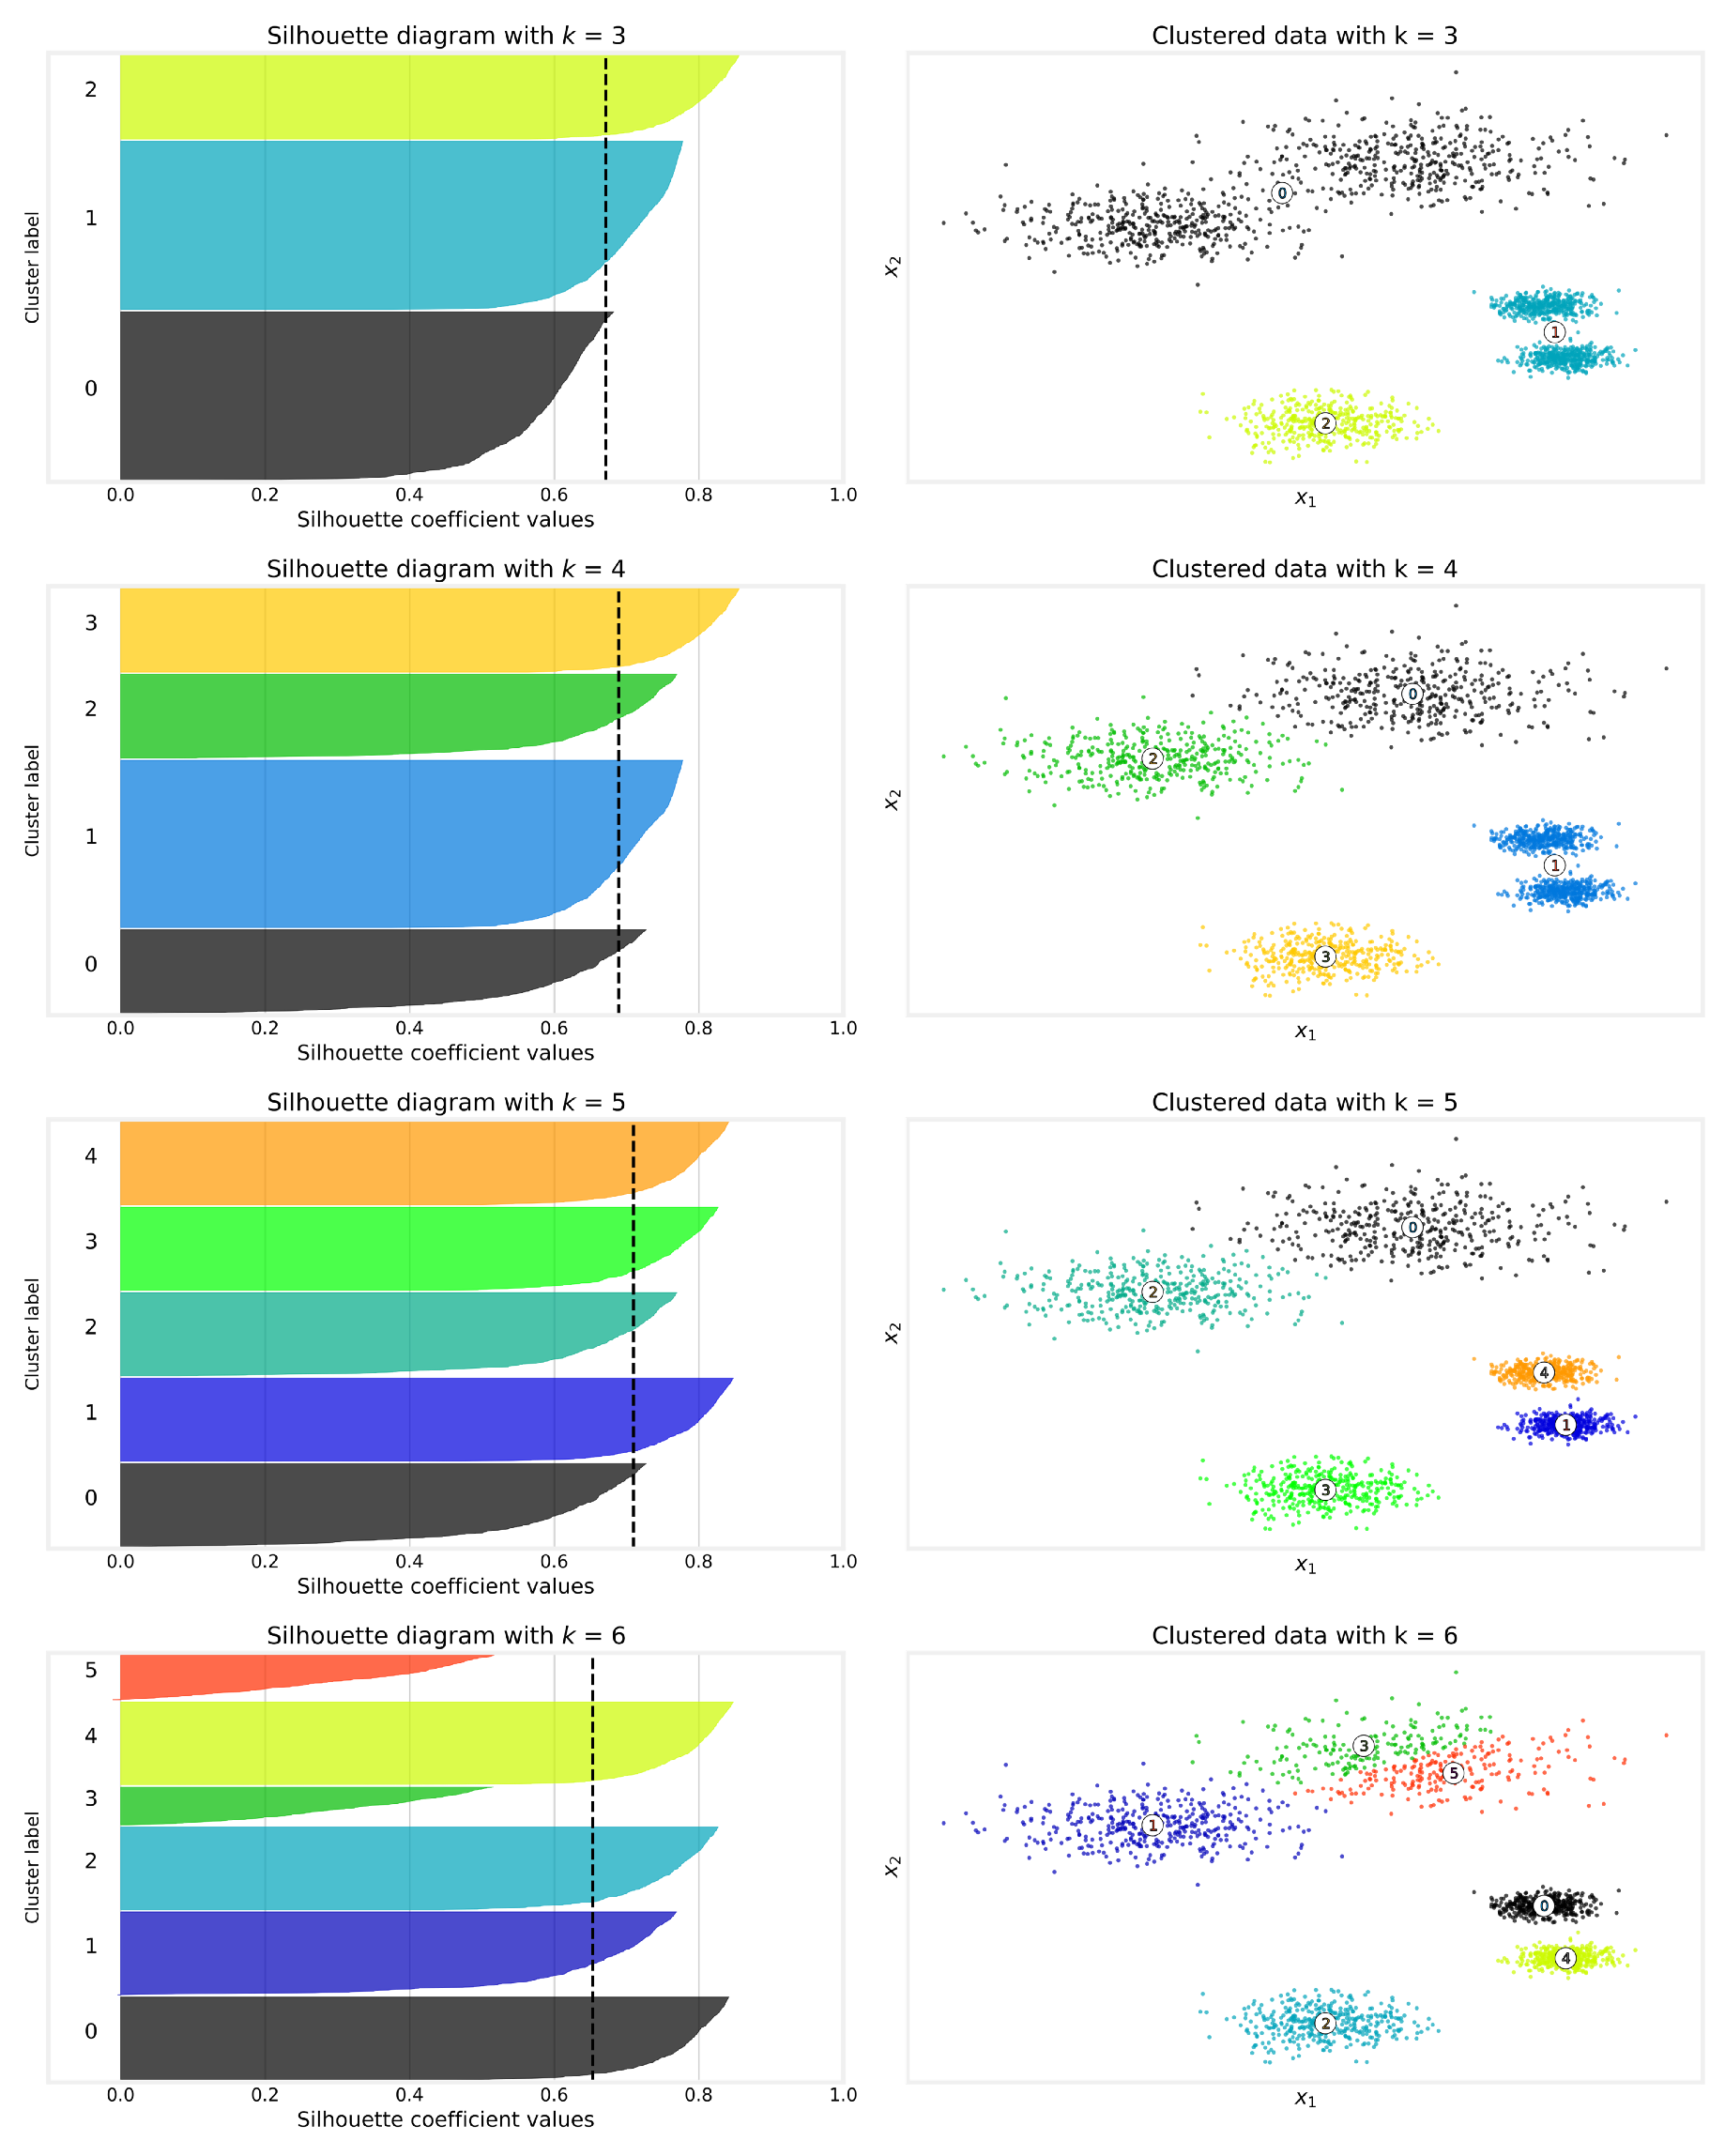
\includegraphics[width=\textwidth]{includes/figures/example_silhouette_plot.png}
\end{example}

\begin{defi}{Prediction Strength}
    Die Idee der \emph{Prediction Strength} ist, dass die  Clusterqualität hoch ist, wenn Clusterzugehörigkeiten auf anderer Realisation der Daten zuverlässig vorhergesagt werden können.

    Das Verfahren ist wie folgt:
    \begin{enumerate}
        \item Zufälliges Aufteilen der Daten $\mathcal{D}$ in zwei Mengen: Trainings- und Validierungsset $\mathcal{D}_\text{train}$ und Validierungsset $\mathcal{D}_\text{val}$.
        \item Clustern der Trainingsdaten und Validierungsdaten separat mit denselben gewählten Parametern.
        \item Ermitteln der Clusterzugehörigkeiten für alle Daten in $\mathcal{D}_\text{val}$ gemäß des Clusterings in $\mathcal{D}_\text{train}$.
        \item Bestimmung des Bruchteils $p$ aller Paare von Datenpunkten in $\mathcal{D}_\text{val}$, die sich auch im selben Cluster in $\mathcal{D}_\text{train}$ befinden würden.
              Der kleinste Wert $p$ über aller Cluster heißt \emph{Prediction Strength}.
    \end{enumerate}

    Sei $M$ eine $N_{\text{val}} \times N_{\text{val}}$-Matrix (\emph{Ko-Mitgliedsschaftsmatrix}) mit
    \[
        M_{i, i'} :=
        \begin{cases}
            1, & \exists k: (i, i') \in R_{C_k} \\
            0, & \text{sonst}
        \end{cases}
    \]
    d. h. ein Matrixeintrag ist 1, wenn die jeweiligen zwei Datenpunkte aus dem Validierungsset zur selben Region eines Clusters $k$ im Trainingset gehören.

    Formal ist die Prediction Strength folgendermaßen definiert:\footnote{$R_{C_k}$ ist die Region des Clusters $k$ im Trainingsset.}
    \[
        \ps(K) = \min_{j = 1, \ldots, K} \frac{1}{|A_j| (|A_j| - 1)} \sum_{i, i' \in A_i, i \neq i'} M_{ii'}
    \]
\end{defi}